
\begin{frame}{malware defenses (1)}
    \begin{itemize}
        \item ``antivirus'' software:
        \vspace{.5cm}
        \item Windows Defender
        \item avast!
        \item Avira
        \item AVG
        \item McAfee
        \item \ldots
    \end{itemize}
\end{frame}

\begin{frame}{malware defenses (2)}
    \begin{itemize}
        \item app stores/etc. filtering (in theory)
            \begin{itemize}
            \item require developer registration
            \item program analysis?
            \item blacklisting after the fact?
            \end{itemize}
        \item ``sandboxing'' policies
            \begin{itemize}
            \item don't let, e.g., game access your taxes
            \item don't let weather app access your microphone
            \end{itemize}
    \end{itemize}
\end{frame}

\begin{frame}[plain]
    \begin{tikzpicture}[remember picture,overlay]
        \node[at=(current page.center)] {
            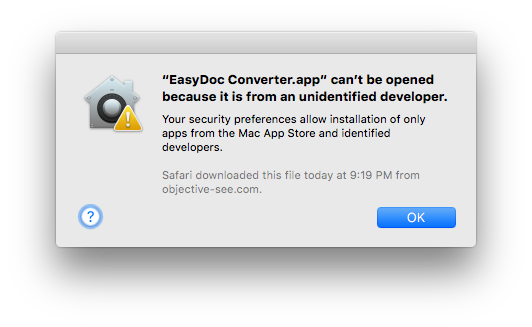
\includegraphics[width=\paperwidth]{../intro/app-denied-mac}
        };
    \end{tikzpicture}
\end{frame}

\begin{frame}[plain]
    \begin{tikzpicture}[remember picture,overlay]
        \node[at=(current page.center)] {
            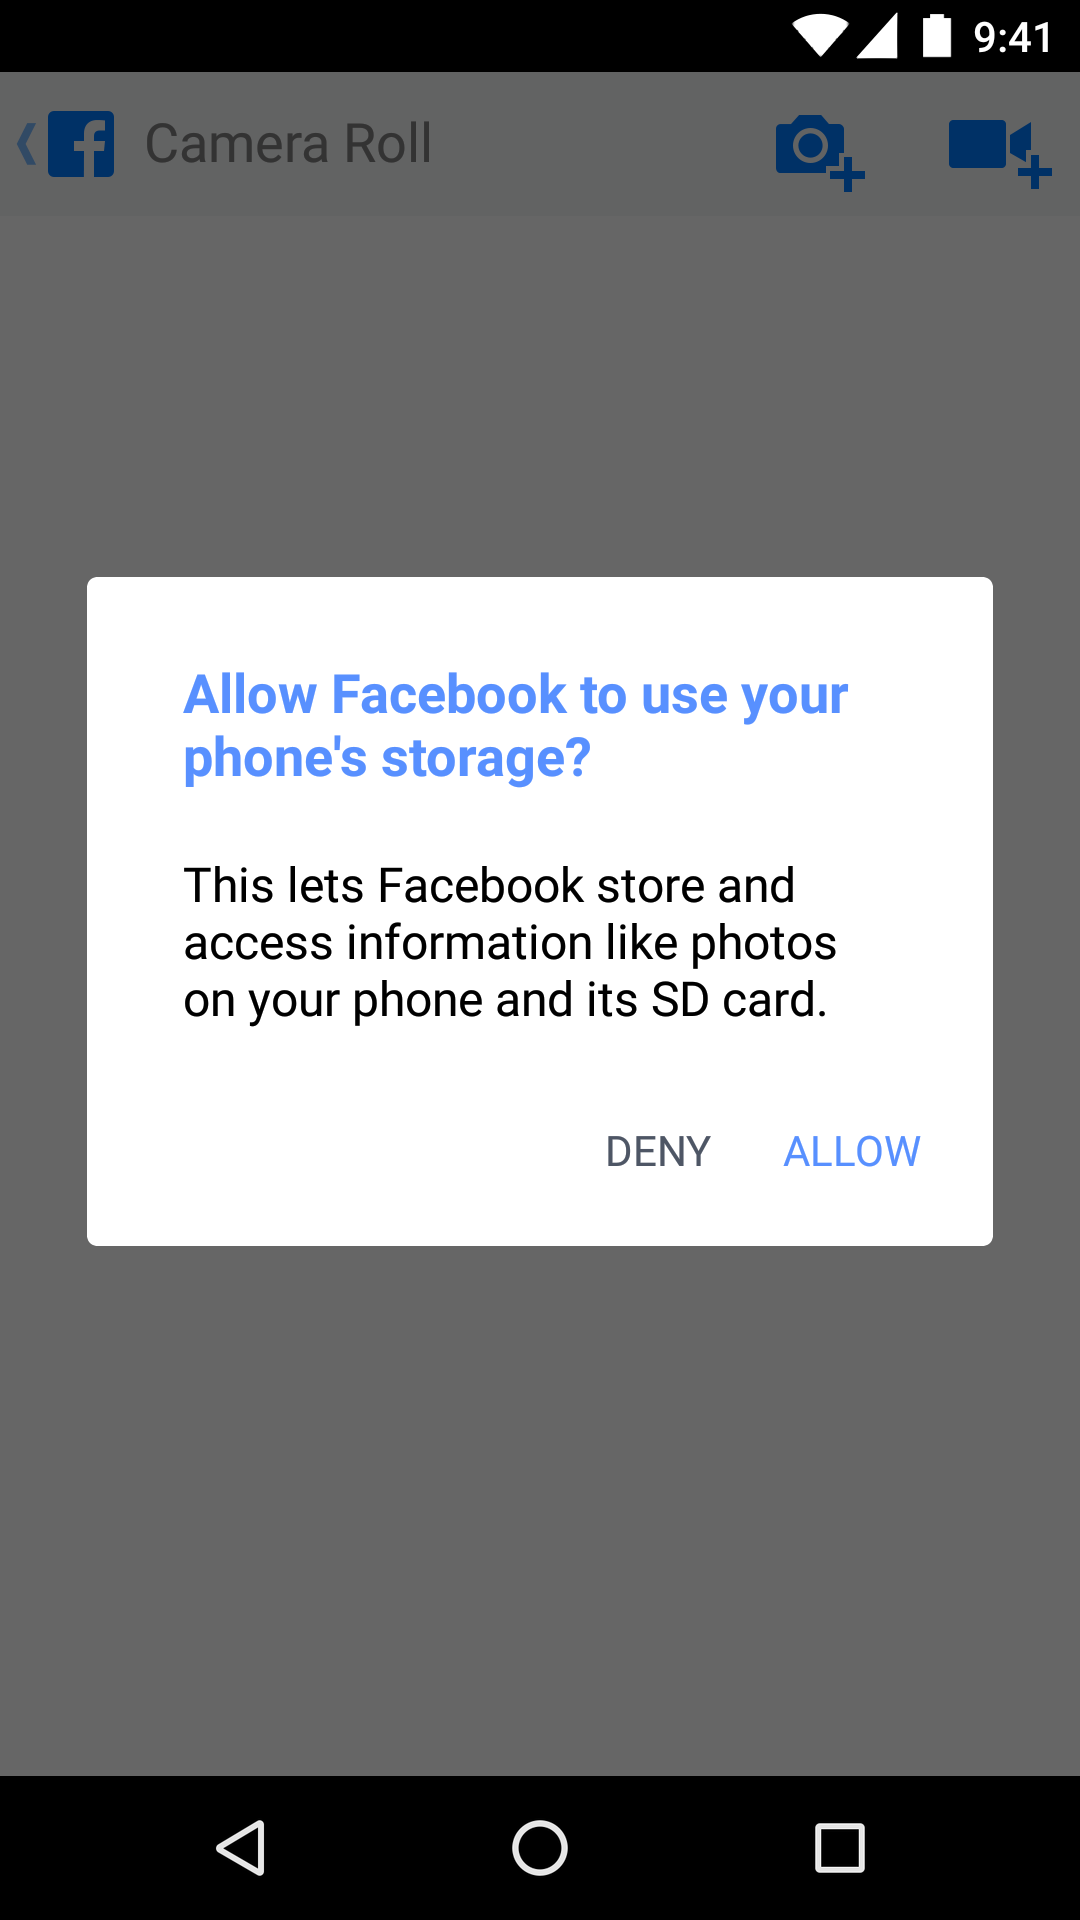
\includegraphics[width=\paperwidth]{../intro/facebook-perms-request}
        };
    \end{tikzpicture}
\end{frame}


\begin{frame}{malware defenses (3)}
    \begin{itemize}
        \item some email spam filters
        \item blacklists for web browsers
            \begin{itemize}
            \item Google Safe Browsing list (Chrome, Firefox)
            \item Microsoft SmartScreen (IE, Edge)
            \end{itemize}
    \end{itemize}
\end{frame}

\begin{frame}{malware counter-defenses}
    \begin{itemize}
    \item malware authors tries to make it hard-to-detect
    \item \myemph{obfuscation}:
        \begin{itemize}
        \item make code \myemph{harder to read}
        \item make code \myemph{different each time}
        \item \myemph{blend in} with normal files/applications/etc.
        \end{itemize}
    \end{itemize}
\end{frame}


